%!TEX root = ../Thesis.tex
\chapter{On the Role of Model Uncertainties in Bayesian Optimization}
\label{chap:UAI}
In this Chapter I present our UAI paper "On the Role of Model Uncertainties in Bayesian Optimization". This project started because Jonathan, a fellow PhD student at DTU, had been applying BO (see Section \ref{sec:BO} for a brief background on BO) in some of his other work and had been pondering on exactly how important surrogate model uncertainty quantification was for BO. I got to know about the project and Jonathan through Michael and Lars Kai and was quickly on-boarded as I had experience in performing BO and was also very interested in the investigation. Although this type of project perhaps does not provide large methodological advances, I think they can be important and useful for the field because they provide guidance for practitioners.\\

\noindent In this work we investigated the impact of model calibration in the context of BO. We did this for a number of surrogate models, including Gaussian Processes (see Section \ref{sec:GPs}), Mean Field Variational Inference BNNs (a special case of VI BNNs presented in Section \ref{sec:BNNs}) and deep ensembles (see Section \ref{sec:DEs}), acquisition functions and across a number of synthetic and real black-box optimisation problems commonly used in BO.  Here we firstly showed that there is correlation between surrogate model calibration and BO performance, i.e. surrogate models that are better calibrated perform better in a BO setting. However, interestingly we found that this association disappeared when controlling for the surrogate model types. Additionally, we were also some of the first to show that DE surrogates perform surprisingly well, at times on par with Gaussian Processes - since then, others have begun to further utilize and investigating BNNs as surrogates in BO \citep{li2024a}. Finally, we also showed both theoretically and empirically that utilizing previously presented recalibration methods \citep{recalibration_BO} during BO may actually lead to \textit{worse} BO performance\footnote{As previously mentioned, please note that \cite{recalibration_BO} has since the time of our UAI paper received several updates and the methods presented herein were not the originally suggested recalibration methods.}. Based on all of these observations and results we presented advice for BO practitioners.

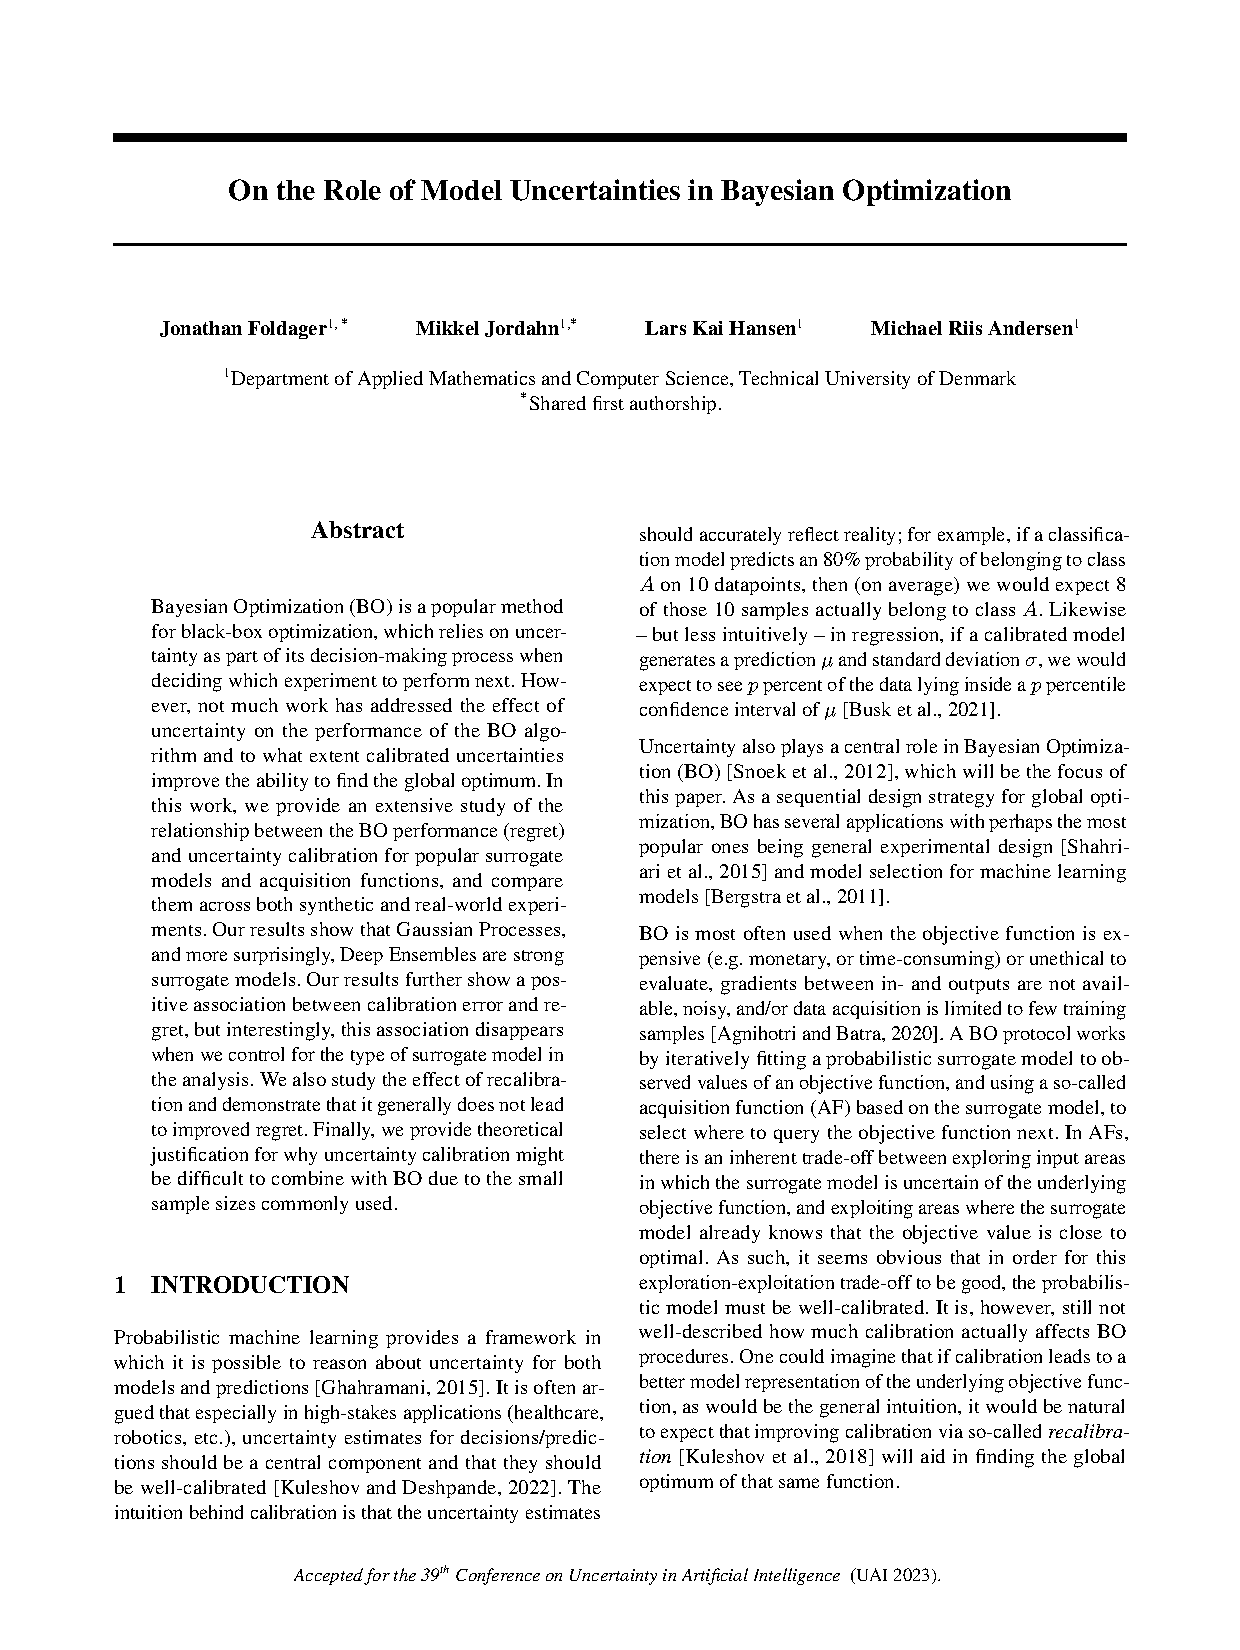
\includepdf[pages=-, offset=0mm -3mm, delta=0mm 0mm, scale=1.0, pagecommand={\thispagestyle{mystuff}{}{}{}}]{chapters/paperC_UAI/UAI_Paper.pdf}
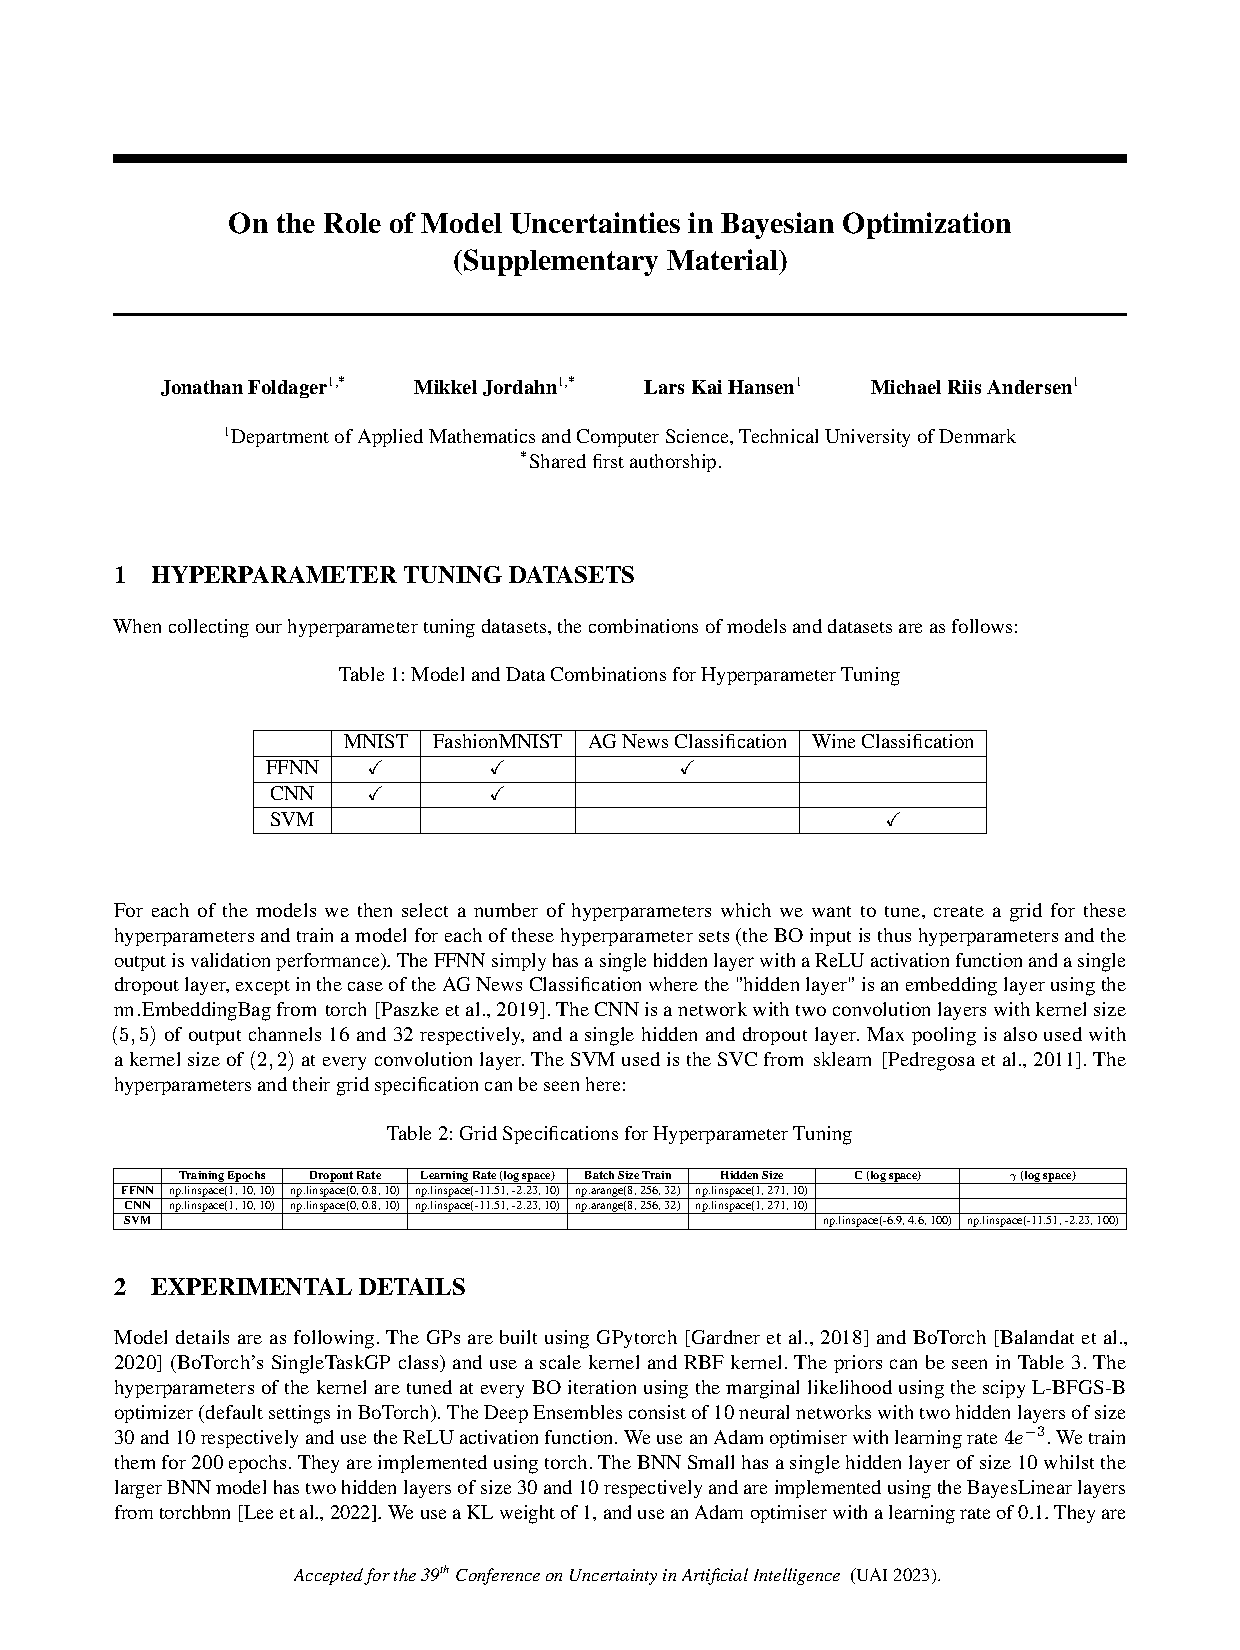
\includepdf[pages=-, offset=0mm -3mm, delta=0mm 0mm, scale=1.0, pagecommand={\thispagestyle{mystuff}{}{}{}}]{chapters/paperC_UAI/UAI_Supp.pdf}